\section{Reconstruction from Multiple Views}%
\label{sec:reconstruction_from_multiple_views}


\subsection{From Two Views to Multiple Views}%
\label{sub:from_two_views_to_multiple_views}


\subsubsection*{Multiple View Geometry}%
\label{ssub:multiple_view_geometry}


In this section, we deal with the problem of 3D reconstruction
given \textbf{multiple} views of a static scene, either obtained simultaneously,
or sequentially from a moving camera.\\

The key idea is that the three-view scenario allows to obtain more measurements
to infer the same number of 3D coordinates.
For example, given two views of a single 3D point, we have four measurements
(x- and y-coordinate in each view), while the three-view case provides
6 measurements per point correspondence.
As a consequence, the estimation of motion and structure will generally
be more constrained when reverting to additional views.\\

The three-view case has traditionally been addressed by the so-called
\textbf{trifocal tensor} [Hartley '95, Vieville '93]
which generalizes the fundamental matrix.
This tensor --- as the fundamental matrix --- does not depend on the scene
structure but rather on the inter-frame camera motion.
It captures a \textbf{trilinear relationship} between three views of
the same 3D point or line [Liu, Huang '86, Spetsakis, Aloimonos '87].


\subsubsection*{Trifocal Tensor versus Multiview Matrices}%
\label{ssub:trifocal_tensor_versus_multiview_matrices}


Traditionally, the trilinear relations were captured by generalizing
the concept of the Fundamental Matrix to that of a Trifocal Tensor.
It was developed among others by [Liu and Huang '86], [Spetsakis, Aloimonos '87].
The use of tensors was promoted by [Vieville '93] and [Hartley '95].
Bilinear, trilinear and quadrilinear constraints were formulated
in [Triggs '95]. This line of work is summarized in the books:
\textbf{Faugeras and Luong, ``The Geometry of Multiple Views'', 2001} and
\textbf{Hartley and Zisserman, ``Multiple View Geometry'', 2001, 2003}.\\

In the following, however, we stick with a matrix notation for the multiview scenario.
This approach makes use of matrices and rank constraints on these matrices
to impose the constraints from multiple views.
Such rank constraints were used by many authors, among othes in [Triggs '95]
and in [Heyden, Astr\"om '97].
This line of work is summarized in the book
\textbf{Ma, Soatto, Kosecka, Sastry, ``An Invitation to 3D Vision'', 2004}.


\subsection{Preimage \& Coimage from Multiple Views}%
\label{sub:preimage_coimage_from_multiple_views}


\subsubsection*{Preimage from Multiple Views}%
\label{ssub:preimage_from_multiple_views}


A \textbf{preimage of multiple images} of a point or a line is the
(largest) set of 3D points that gives rise to the same set of
multiple images of the point or the line.\\

For example, given the two images $l_1$ and $l_2$ of a line $L$,
the preimage of these two images is the intersection of the planes
$P_1$ and $P_2$, i.e.\ exactly the 3D line $L = P_1 \cap P_2$.\\

In general, the preimage of multiple images of points and lines
can be \textbf{defined by the intersection}:
\[
	\preim (a_1, \ldots, a_m) = \bigcap_{i = 1, m} \preim (a_i)
\]
The preimage of multiple image lines or points can be either
an empty set, a point, a line or a plane.

\begin{figure}[h]
	\centering
	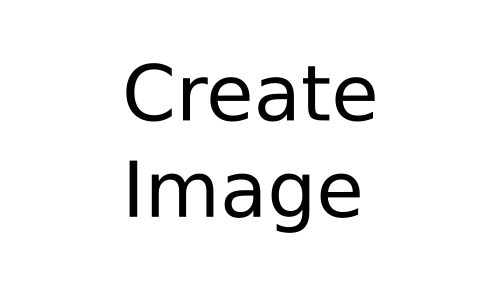
\includegraphics[width=\linewidth]{img/todo.png}
	\caption{Preimage and coimage of points and lines. (video 10, minute 34)}%
	\label{fig:preimage_coimage}
\end{figure}

Figure~\ref{fig:preimage_coimage} shows the preimage and coimage of a point $p$
on a line $L$.
\begin{itemize}
	\item Preimages $P_1$ and $P_2$ of the image lines should intersect on the line $L$.
	\item Preimages of the two image points $\bm{x}_1$ and $\bm{x}_2$
		should intersect in the point $p$.
	\item Normals $l_1$ and $l_2$ define the coimages of the line $L$.
\end{itemize}


\subsubsection*{Preimage and Coimage of Points and Lines}%
\label{ssub:preimage_and_coimage_of_points_and_lines}

For a \textbf{moving camera at time $t$}, let $\bm{x}(t)$ denote the image coordinates
of a 3D point $\bm{X}$ in homogeneous coordinates:
\[
	\lambda(t) \bm{x}(t) = K(t) \Pi_0 g(t) \bm{X}
\]
where $\lambda(t)$ denotes the depth of the point, $K(t)$ the intrinsic parameters,
$\Pi_0$ the generic projection, and
\[
	g(t) = \begin{pmatrix}
		R(t) & T(t) \\
		0 & 1
	\end{pmatrix}
	\in SE(3)
\]
denotes the rigid body motion at time $t$.
Let us consider a \textbf{3D line $L$} in homogeneous coordinates:
\[
	L = \Set {\bm{X}} {\bm{X} = \bm{X}_0 + \mu \bm{V}, \mu \in \R} \subset \R^4
\]
where $\bm{X}_0 = \tr{[ X_0, Y_0, Z_0, 1 ]} \in \R^4$ are the coordinates
of the base point $p_0$ and the vector $\bm{V} = \tr{[V_1, V_2, V_3, 0]} \in \R^4$
is a nonzero vector indicating the line direction.\\

The \textbf{preimage of $L$} with respect to the image at time $t$ is a plane $P$
with normal $l(t)$, where $P = \text{span}(\widehat{l})$.
The vector $l(t)$ is orthogonal to all points $\bm{x}(t)$ of the line:
\[
	\tr{l(t)} \bm{x}(t) = \tr{l(t)} K(t) \Pi_0 g(t) \bm{X} = 0
\]
Assume we are given a \textbf{set of $m$ images at times} $t_1, \ldots, t_m$
where
\[
	\lambda_i = \lambda(t_i),
	\bm{x}_i = \bm{x}(t_i),
	l_i = l(t_i),
	\Pi_i = K(t_i) \Pi_0 g(t_i)
\]
With this notation, we can relate the \textbf{$i$-th image of a point $p$}
to its world coordinates $\bm{X}$:
\[
	\lambda_i \bm{x}_i = \Pi_i \bm{X}
\]
and the \textbf{$i$-th coimage of a line $L$}
to its world coordinates $(\bm{X}_0, \bm{V})$:
\[
	\tr{l_i} \Pi_i \bm{X}_0 = \tr{l_i} \Pi_i \bm{V} = 0
\]


\subsection{From Preimages to Rank Constraints}%
\label{sub:from_preimages_to_rank_constraints}


The above equations contain the \textbf{3D parameters of points and lines}
as unknowns. As in the two-view case, we wish to
\textbf{eliminate these unknowns} so as to obtain relationships between
the 2D projections and the camera parameters.\\

In the two-view case an elimination of the 3D coordinates lead to the
\textbf{epipolar constraint} for the essential matrix $E$ or
(in the uncalibrated case) the fundamental matrix $F$.
The 3D coordinates (depth values $\lambda_i$ associated with each point)
could subsequently be obtained from another contraint.\\

There exist \textbf{different ways to eliminate the 3D parameters}
leading to different kinds of constraints which have been studied in Computer Vision.\\

A systematic elimination of these constraints will lead to a complete set of conditions.


\subsubsection*{Point Features}%
\label{ssub:point_features}

Consider images of a 3D point $\bm{X}$ seen in multiple views:
\[
	\I \lambda \equiv
		\begin{pmatrix}
			\bm{x}_1 & 0 & \cdots & 0 \\
			0 & \bm{x}_2 & \cdots & 0 \\
			\vdots & \vdots & \ddots & \vdots \\
			0 & 0 & \cdots & \bm{x}_m
		\end{pmatrix}
		\begin{pmatrix}\lambda_1 \\ \lambda_2 \\ \vdots \\ \lambda_m \end{pmatrix}
		= \begin{pmatrix}\Pi_1 \\ \Pi_2 \\ \vdots \\ \Pi_m \end{pmatrix} \bm{X}
\]
which is of the form
\[
	\I \lambda = \Pi \bm{X}
\]
where $\lambda \in \R^m$ is the \textbf{depth scale vector},
and $\Pi \in \RR{3m}{4}$ the \textbf{multiple-view projection matrix}
associated with the \textbf{image matrix} $\I \in \RR{3m}{m}$.\\

Note that apart from the 2D coordinates $\I$, everything else in the above
equations is unknown. As in the two-view case, the goal is to decouple
the above equation into constraints which allow to separately recover
the camera displacements $\Pi_i$ on one hand and the scene
structure $\lambda_i$ and $\bm{X}$ on the other hand.\\

Every column of $\I$ lies in a four-dimensional space spanned by colummns
of the matrix $\Pi$. In order to have a solution to the above equation,
the columns of $\I$ and $\Pi$ must therefore be linearly dependent,
in other words, the matrix
\[
	N_p \equiv (\Pi, \I)
	= \begin{pmatrix}
		\Pi_1 & \bm{x}_1 & 0 & \cdots & 0 \\
		\Pi_2 & 0 & \bm{x}_2 & \cdots & 0 \\
		\vdots & \vdots & \vdots & \ddots & \vdots \\
		\Pi_m & 0 & 0 & \cdots & \bm{x}_m
	\end{pmatrix}
\]
where $N_p \in \RR{3m}{(4+m)}$, must have a nontrivial right null space.
For $m \geq 2$ (i.e. $3m \geq m + 4$), full rank would be $m+4$.
Linear dependence of columns therefore implies the \textbf{rank constraint}:
\[
	\boxed{\text{rank}(N_p) \leq m + 3 }
\]
In fact, the vector $u \equiv \tr{( \tr{\bm{x}}, - \tr{\lambda} )} \in \R^{m+4}$
is in the right null space, since $N_p u = 0$.\\

For a more compact formulation of the above rank constraint,
we introduce the matrix
\[
	\I^{\bot} \equiv
		\diagtwo{\widehat{\bm{x}_1}}{\widehat{\bm{x}_m}}
		\in \RR{3m}{3m}
\]
which has the property of ``annihilating'' $\I$:
\[
	\I^{\bot} \I = 0
\]
We can premultiply the above equation to obtain
\[
	\I^{\bot} \Pi \bm{X} = 0
\]
Thus the vector $\bm{X}$ is in the null space of the matrix
\[
	W_p
		\equiv \I^{\bot} \Pi
		= \begin{pmatrix}
			\widehat{\bm{x}_1} \Pi_1 \\ \vdots \\ \widehat{\bm{x}_m} \Pi_m
		\end{pmatrix}
		\in \RR{3m}{4}
\]
To have a nontrivial solution, we must have
\[
	\text{rank}(W_p) \leq 3
\]
If all images $\bm{x}_i$ are from a single 3D point $\bm{x}$,
then the matrix $W_p$ should only have a one-dimensional null space.
Given $m$ images $\bm{x}_i \in \R^3$ of a point $p$ with respect to $m$ camera
frames $\Pi_i$, we must have the rank condition
\[
	\boxed{\text{rank}(W_p) = \text{rank}(N_p) - m \leq 3}
\]


\subsubsection*{Line Features}%
\label{ssub:line_features}

We can derive a similar rank constraint for lines.
As we saw above, for the coimages $l_i, i=1, \ldots, m$ of a line $L$
spanned by a base $\bm{X}_0$ and a direction $\bm{V}$ we have:
\[
	\tr{l_i} \Pi_i \bm{X}_0 = \tr{l_i} \Pi_i \bm{V} = 0
\]
Therefore the matrix
\[
	W_l \equiv \begin{pmatrix}
		\tr{l_1} \Pi_1 \\ \vdots \\ \tr{l_m} \Pi_m
	\end{pmatrix}
	\in \RR{m}{4}
\]
must satisfy the rank constraint
\[
	\boxed{\text{rank}(W_l) \leq 2}
\]
since the null space of $W_l$ contains the two vectors $\bm{X}_0$ and $\bm{V}$.


\subsection{Geometric Interpretation}%
\label{sub:geometric_interpretation}


\subsubsection*{Rank Constraints: Geometric Interpretation}%
\label{ssub:rank_constraints_geometric_interpretation}

In the case of a \textbf{point} $\bm{X}$, we had the equation
\[
	W_p \bm{X} = 0, \quad \text{with} \quad
	W_p = \begin{pmatrix}
			\widehat{\bm{x}_1} \Pi_1 \\ \vdots \\ \widehat{\bm{x}_m} \Pi_m
		\end{pmatrix}
		\in \RR{3m}{4}
\]
Since all matrices $\widehat{\bm{x}_i}$ have rank 2, the number of independent
rows in $W_p$ is at most $2m$. These rows define a set of $2m$ planes.
Since $W_p \bm{X} = 0$, the point $\bm{x}$ is in the intersection of all these planes.
In order for the $2m$ planes to have a unique intersection,
we need to have $\text{rank}(W_p) = 3$.\\

In the case of a line $L$ in two views, we have the equation
\[
	\text{rank}(W_l) \leq 2, \quad \text{with} \quad
	W_l = \begin{pmatrix}
		\tr{l_1} \Pi_1 \\ \tr{l_2} \Pi_2
	\end{pmatrix}
	\in \RR{2}{4}
\]
Clearly, we already have $\text{rank}(W_l) \leq 2$, so there is no intrinsic
constraint on two images of a line: The preimage of two image lines
always contains a line. We shall see that this is no longer true for three
or more images of a line, then the above constraint really becomes meaningful.


\subsection{The Multiple-View Matrix}%
\label{sub:the_multiple_view_matrix}


\subsection{Relation to Epipolar Constraints}%
\label{sub:relation_to_epipolar_constraints}


\subsection{Multiple-View Reconstruction Algorithms}%
\label{sub:multiple_view_reconstruction_algorithms}


\subsection{Multiple-View Reconstruction of Lines}%
\label{sub:multiple_view_reconstruction_of_lines}


